\section{Model}\label{sec:Model}
In this section we describe the model that is used to find the speed that will let a vehicle arraive at the next traffic light as it turns green.
See Figure~\ref{fig:Introduction:network} for references.

\subsection{Vehicles}
A vehicle, $\veh$, is an entity that moves along a route.
Each vehicle has an identifier, $\vehid$, a constant acceleration, $\vehacc$ and deceleration, $\vehdec$ and a current position, \vehpos. 
The position is either an edge or a connection (see Section~\ref{sec:map}).
The position is updated as the vehicle moves.
For simplicity we do not consider different drivering behaviours, and operate with one type of vehicle. 

\subsection{Map}\label{sec:map}
A map is a directed graph, $G = (V, E, C)$ where $V$ is a set of vertices, $E$ is a set of edges representing road segments and $C$ is a set of connections between edges.
An egde represents one direction of a road segment.
Every edge $\edge\in E$ has a starting point $\estart\in V$, an end point $\eend\in V$ and a maximum speed $\espeed\in\mathbb{R}$. 
The lenght of an edge is the euclidean distance between $\estart$ and \eend denoted as \elength.
In Figure~\ref{fig:Introduction:network} we have five egdes: two to the west of traffic light, two to the east and one to the north.

By connecting edges through connections, it is possible to model exactly the possible paths through a junction - for example disallowing a right turn.
A connection is also associated a traffic light phase, $\cphase$ detailing when this connection has a red, green or yellow signal (see Section~\ref{sec:phases}).
A juction is therefore made up of several connections that connect the road segments that one can drive to and from.
For example each possible legal pass through the intersection in Figure~\ref{fig:Introduction:network} is a connection as shown in Figure~\ref{fig:Model:Connection} as red arrows. 
A connection, $\con$ is hence unidirectional from one vertex, $\cestart\in V$ to another vertex, $\ceend \in V$, and a connection is made for each lane of the edges.
The example in Figure~\ref{fig:Introduction:network} hence have six connections assuming one cannot make U-turns.
Connections can be seen as a type of edge associated with a phase.
With this abstraction, it is possible to use standard route computing algorithms such as Dikstra's algorithm or A*.

\begin{figure}[h]
\centering
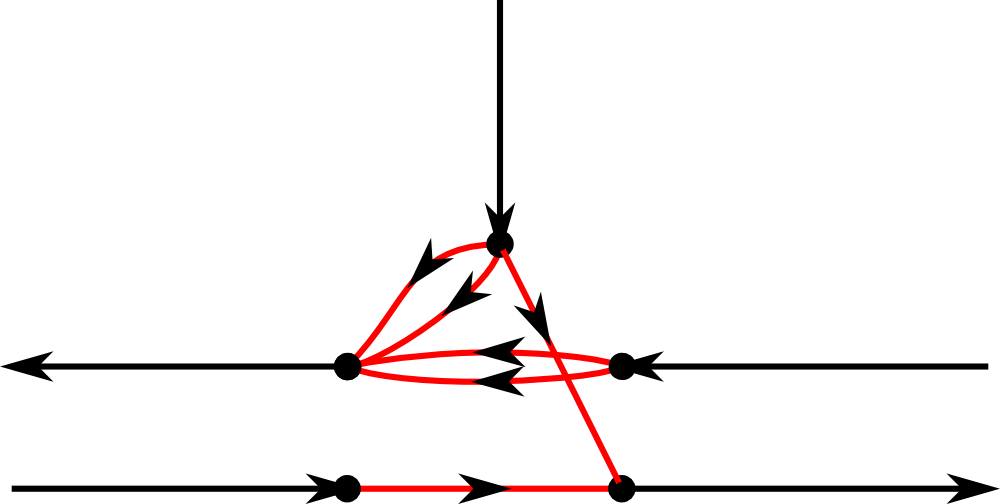
\includegraphics[width=0.4\textwidth]{../images/ConnectionNetwork.png}
\caption{Connection network of Figure \ref{fig:Introduction:network}}
\label{fig:Model:Connection}
\end{figure}

\begin{comment}
\subsection{Sensors}
A sensor can detect whether a vehicle is located at the sensor or not. 
Sensors can for example be induction loops or video cameras.
We only use induction loops, that register when a vehicle is directly on top of it. 
An induction loop, $\indLoop\in\indLoopSet$, has a position, \indLoopPos which is the distance to the associated traffic light, a location, \indLoopLoc which is the lane it is located at and a vehicle count, $\indLoopVeh\in \mathbb{N}_0$ being the number of vehicles currently at the induction loop.
\end{comment}

\subsection{Traffic Light Phases}\label{sec:phases}
Each connection in a traffic light has a phase that details the light setting for just this one connection.
SUMO limits the allowed light settings to $red$, $yellow$ and $green$.
A phase of a traffic light, $\phase$ is defined as $\langle(\light_0, \ti_0),(\light_1, \ti_1),\dots, (\light_n, \ti_n) \rangle$ where $t_i>0$ and the light setting is $\light_i\in \{red, yellow, green\}$ in $\ti_i$ seconds for $0 \leq i \leq n$.
There must exist at least one occurence where $\light_i = green$ for $i \in \{0 \dots n\}$. 
A connection in an unregulated junction will simply have the phase $\langle(green, \infty)\rangle$.
Let $\Ccirc{\phase} = \sum_{i=0}^{n}\ti_i$ be the circulation time of \phase where $(\light_i, \ti_i)\in \phase$.
A typical circulation time of a phase is between $35$ to $80$ seconds but can up to $110$ seconds. 
The yellow periodes are often $4s$ before a red periode and $2s$ before a green period\cite{vejtrafik}.

\subsection{Junction}
We define a junction \ju to be a set of connections, $\jucons \subseteq C$. 
A junction can be either regulated or unregulated. 
In an unregulated traffic light traffic must give way to traffic coming from the right. 
In a regulated traffic light vehicles will have to check the phase $\cphase$ of the connection \vehpos. 
A junction is said to be unregulated iff $\forall c \in \jucons | \cphase = \langle(green, \infty)\rangle$

\subsection{Routes}
A route, $\route$, is a sequence of edges on the map, $\langle \edge_0, \edge_1, \dots \edge_n \rangle$, where $\exists \con$ such that $\eendi{i} = \cestart$ and $\estarti{i+1} = \ceend$ for $0\leq i< n$.
The vehicle starts at $\edge_0$ and moves along the sequence until $\edge_n$ has been reached.





